\chapter{Methodology}

%%%%%%%%%%%%%%%%%%%%%%%%%%%%%%%%%%%%%%%%%%%%%%%%%%%%%%%%%%%%%%%

\begin{figure}
\centering
\includegraphics[width=0.9\textwidth]{batt_model}
\caption{Battery model for simulation.}
\label{fig:batt_model}
\end{figure}

The parameters of the model are [need source]
\begin{align}
	R_s &= 0.1562 e^{-24.37 V_{SOC}} + 0.07446 \\
	R_{ts} &= 0.3208 e^{-29.14 V_{SOC}} + 0.04669 \\
	C_{ts} &= -752.9 e^{-13.51 V_{SOC}} + 703.6 \\
	R_{tl} &= 6.603 e^{-155.2 V_{SOC}} + 0.04984 \\
	C_{tl} &= -6056 e^{-27.12 V_{SOC}} + 4475 \\
	V_{OC} &= -1.031 e^{-35 V_{SOC}} + 3.685 + 0.2156 V_{SOC} - 0.1178 V_{SOC}^2 + 0.3201 V_{SOC}^3
\end{align}

The corresponding state space model is
\begin{gather}
	x = \left[ v_{C_{ts}} \quad v_{C_{tl}} \quad V_{OC} \right] \\
	\dot{x} = \begin{bmatrix}
		-1/R_{ts}C_{ts} & 0 & 0 \\
		0 & -1/R_{tl}C_{tl} & 0 \\
		0 & 0 & 0
		\end{bmatrix} x 
		+ \begin{bmatrix} 1/C_{ts} & 1/C_{tl} \end{bmatrix} i_\text{cell} \\
	v_\text{cell} = [-1 \quad -1 \quad 1] x - R_s i_\text{cell}
\end{gather}

\begin{figure}
\centering
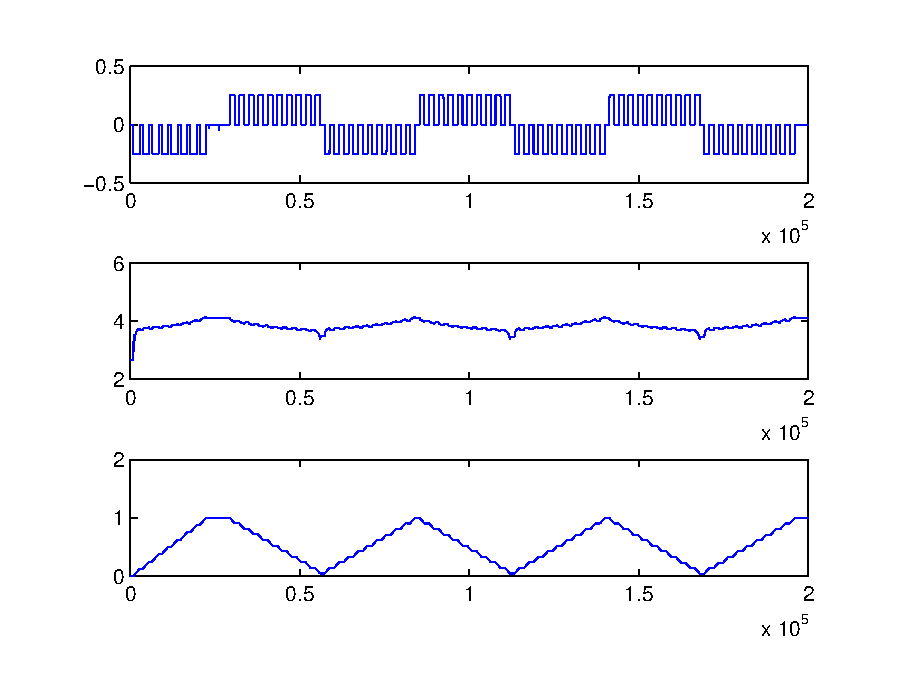
\includegraphics[width=0.9\textwidth]{sim_ideal}
\caption{Discharge current along with the resulting voltage and SOC.}
\label{fig:idealsim}
\end{figure}
